\documentclass[12pt]{article}
\usepackage[utf8]{inputenc}
\usepackage{cite}
\usepackage[portuguese]{babel}
\usepackage{natbib}
\usepackage{graphicx}
\usepackage{url}



\title{FI582 - FÍSICA PARA COMPUTAÇÃO}
\author{Pedro Calheiros de Araujo}
\date{Abril, 2022}

\begin{document}

\maketitle

\begin{figure}[h!]
\centering
    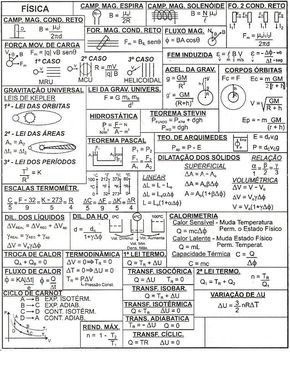
\includegraphics[width=80mm]{formulas.jpeg}
    \caption{Formulas usadas em Fisica para Computação. \cite{img:graph}}
    \label{fig:graph1}
\end{figure}

\section{Introdução}
\par 
A cadeira de Física para Computação, compila os assuntos dados em FI006 - FÍSICA GERAL 1, FI007 - FÍSICA GERAL 2 e FI008 - FÍSICA GERAL 3, como: revisão de mecânica; eletricidade; eletromagnetismo; oscilações; ondas; conceitos de termodinâmica; entre outros. Alguns deles já abordados no Ensino Médio. É uma disciplina que busca discutir os principais tópicos da física clássica e relacioná-los com a teoria computacional, assim dando uma base para uma futura aplicação de tais conceitos em outros ambientes. Na UFPE, no curso de Ciência da Computação, Física para Computação é uma cadeira obrigatória do segundo período, atualmente é ministrada pelo professor Azadeh Mohammed, suas aulas presenciais ocorrem no CCEN (Centro de Ciências Exatas e da Natureza) na sala D005. A bibliografia utilizada pelo professor consiste no livro Physics for Computer Science Students: With Emphasis on Atomic and Semiconductor Physics. Narciso García, A. C. Damask, Steven Schwarz. Spinger, 1998.
\cite{fonte:xxx}
\cite{fonte:yyy}
\cite{fonte:zzz}
\cite{fonte:www}

\section{Relevância}
\par
Nos primórdios do estudo computacional a física na computação era muito mais relevante que nos dias atuais, uma vez que o avanço tecnológico dos componentes físicos dos computadores limitava o avanço da ciência da computação em geral. Esse não é mais o caso devido a constante miniaturização do \textit{hardware} dos computadores. Porém a Física ainda é muito importante para a computação como um todo, visto que apresenta conceitos que são úteis em diversas áreas como: visualização computacional, processamento de sinais, inteligência artificial, simulação, processamento de imagens, criação de jogos, entre outras. Além de dar uma ampla noção de aplicações e conceitos do mundo real, que podem ser de grande utilidade.
\cite{fonte:zzz}
\cite{fonte:www}

\section{Relações com outras disciplinas}
\par
Apesar de não ser pré-requisito para nenhuma cadeira e de ter apenas um co-requisitos: MA026 - CALCULO DIFERENCIAL E INTEGRAL 1, Física para Computação é extremamente importante para demais cadeiras e para a formação de um cientista da computação. Portanto, é paga logo no segundo período porque possui conceitos e ensina raciocínios que serão usados direta e indiretamente em diversas outras disciplinas no futuro como: IF752 - ANÁLISE IMAG. VISÃO COMPUTACIONAL, IF750 - COMPUTAÇÃO GRAFICA, IF728 - ENGENHARIA DE SISTEMAS EMBUTIDOS, entre outras. Além disso, ela é a ponte para outras áreas do saber, já que abrange temas que vão além do \textit{software} se comunicando até com outros cursos como as engenharias, possuindo como equivalente acadêmica: FI108 - FISICA GERAL 3.
\cite{fonte:yyy}


\bibliographystyle{plain}
\bibliography{bbg.bib}

\end{document}